\documentclass[10pt]{article}
\usepackage{graphicx}
\usepackage{hyperref}
\hypersetup{colorlinks,breaklinks,
            urlcolor=[rgb]{0,0,0},
            citecolor=[rgb]{0,0,0},
            linkcolor=[rgb]{0,0,0}}
\usepackage{fullpage}
\setlength{\parindent}{0em}
\setlength{\parskip}{1.0em}
\linespread{1}
\usepackage[table]{xcolor}
\usepackage{times}
% \usepackage[bitstream-charter]{mathdesign}
\usepackage[T1]{fontenc}
\bibliographystyle{unsrt}
\newcommand{\tion}[1]{\textsection\ref{sect:#1}}

\begin{document}
% Title Space
\title{\textsc{Evolutionary Multi-Objective Optimization:\\ A Distributed Computing approach}}
\author{Rahul Krishna (\textbf{rkrish11}) \hspace{0.75cm} George Mathew (\textbf{george2}) \\Dept. Computer Science\\North Carolina State University}
\date{}
\maketitle
% Abstract
\section*{Abstract}

Optimization is the task of finding one or more solutions which satisfy one or more specified objectives. While a single-objective optimization involves a single objective function and a single solutions, a multi-objective optimization considers several objectives simultaneously. In such a  case, a multi-objective optimizer generates a set of alternate solution with certain trade-offs. These are called Pareto optimal solutions.

Multi-objective problems are usually complex, NP-Hard, and resource intensive. Although exact methods can be used, they consume prohibitively large amounts of time and memory. An alternative approach would be to make use of meta-heuristic algorithms, which approximate the Pareto frontier in a reasonable amount of time. Even so, these meta-heuristic algorithms consume a significant amount of time. 

Parallel and distributed computing used in design and implementation of these algorithms may offer significant speed-ups. In addition to this, they may be used to improve the quality, increase the robustness of the the obtained solutions, and may also allow the algorithms to be scaled to solve large problems. 

In this project, we aim to present parallel models for two evolutionary multi-objective optimizers: (1) Differential Evolution (DE) \cite{storn97}; and (2) Geometric Active Learning (GALE) \cite{krall15}. From the implementation point of view, we focus on using the \textit{henry2 Linux cluster} offered by NC State with distributed programming environments such as message passing (OpenMPI)~\cite{openMPI04}.

This report is organized as follows. The following section presents a brief description of the algorithms being studied. In \textsection\ref{measures}, we discuss various methods for evaluating the performance of the parallelized algorithms. In section \textsection\ref{challenges}, we highlight challenges we expect to overcome during implementation. Finally, section \textsection\ref{tools} highlights the tools we use.

\section{Evolutionary Algorithms}
\label{algos}

An Evolutionary Optimization(EO) begins its search with a population of solutions usually created at random within a specified lower and upper bound on each variable. If bounds are not supplied in an optimization problem, suitable values can be assumed only for the initialization purpose. Thereafter, the EO procedure enters into an iterative operation of updating the current population to create a new population by the use of four main operators: selection, crossover, mutation and elite-preservation. The operation stops when one or more pre-specified termination criteria are met. The following evolutionary algorithms shall be parallelized.
\begin{enumerate}
\item \textbf{Differential Evolution (DE):} Differential evolution is a stochastic and population based optimization technique that iteratively tries to improve a candidate solution with respect to measure of quality. An objective function is defined in a selected region of the problem space. A candidate solution is then optimized to minimize/maximize the objective function based on the nature of the problem. Differential evolution offers the following advantages:

\begin{itemize}
\item It is computationally inexpensive.
\item It can handle problems with a high dimensionality. 
\item It allows the user to understand how the current solution was generated.
\end{itemize}

\item \textbf{Geometric Active Learning (GALE):} GALE is a near-linear time multi-objective optimization algorithm that builds a piecewise approximation to the surface of best solutions along the Pareto frontier. GALE uses a clustering algorithm called WHERE, which is powered by a FASTMAP \cite{faloutsos95}, to recursively reduce the dimensions to a single principal component. GALE offers the following advantages:

\begin{itemize}
\item It optimizes a problem with far fewer computations compared to other algorithms.
\item It is particularly adept at handling objective functions that are non-differentiable, non-linear, multidimensional, or are subject to multiple constraints.
\item It offers a very concise representation of the problem space due to WHERE.
\end{itemize}
\end{enumerate}

\section{Optimization Problem}
\label{problem}

Multi-objective Evolutionary Algorithms(MOEA) require scalable test problems that help test its efficiency. Our chosen test problem is a mathematical test problem \textbf{DTLZ2} \cite{debMOEA02}, which was formulated by \textit{Kalyanmoy \textbf{D}eb}, \textit{Lothar \textbf{T}hiele}, \textit{Marco \textbf{L}aumans} and \textit{Eckhart \textbf{Z}itzler}. 

\textbf{Decisions} : DTLZ2 has 30 decisions between 0 and 1.
\[0 \leq {x}_{i} \leq 1 \ \ \ \ where \ \  i = 1,2 ,3 .... 30\]

\textbf{Objectives} : Although DTLZ2 allows as to generate upto n-1 objectives where n is the number of decisions, we choose to limit the number of objectives to 3 since we can model the objectives better to visualize the pareto frontier. Limiting the number of objectives also controls the domination pressure. All the three objectives needs to be minimized. The objectives are defined as follows:
\[{f}_{1}(x) = (1+g({x}_{M}))\cos({x}_{1} \pi/2)....\cos({x}_{M-1} \pi/2)\]
\[{f}_{2}(x) = (1+g({x}_{M}))\cos({x}_{1} \pi/2)....\cos({x}_{M-1} \pi/2)\]
\[{f}_{3}(x) = (1+g({x}_{M}))\sin({x}_{1} \pi/2)\]
\[where \ \ \ \ g({x}_{M}) = \sum_{x \in {x}_{M}} (x_i - 0.5)^2 \]

\textbf{Optimal Solutions} : The pareto optimal solutions corresponds to the decisions \(x_i = 0.5\) and all objective function values must satisfy \(\sum_{m=1}^M (f_m)^2 = 1\). Figure \ref{fig:problem} shows the pareto frontier that represents the optimal solutions of DTLZ2.

\begin{figure}
\centering
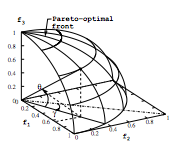
\includegraphics{img/dtlz2_pareto.png}
\caption{Pareto Frontier of DTLZ2}
\label{fig:problem}
\end{figure}





\section{Measures}
\label{measures}
Figure \ref{fig:measure} highlights some of the performance evaluation measures we use to evaluate the algorithms.

\begin{figure}[h!]
\begin{tabular}{ll}
\hline
\rowcolor[HTML]{EFEFEF} 
\multicolumn{1}{l}{\cellcolor[HTML]{EFEFEF}{\bf Measure}} & \multicolumn{1}{c}{\cellcolor[HTML]{EFEFEF}{\bf  Description}}                                                                                                                                                                                                                                                                    \\ \hline
\rowcolor[HTML]{FFFFFF} 
{\bf Runtime}                                             & Time taken for the algorithm to be generate optimal solutions.\\
{\bf Convergence}                                         & \begin{tabular}[l]{@{}l@{}}Convergence is the accuracy of the obtained solutions. It mathematically represents \\ the hypervolume of the Pareto frontier. In case of a minimization problem, we expect \\ it to be less and large in the case of a maximization problem.\end{tabular} \\
\rowcolor[HTML]{FFFFFF} 
{\bf Diversity}                                           & \begin{tabular}[l]{@{}l@{}}Diversity represents the spread of the proposed solutions. Ideally the solutions should \\ be well distributed across the Pareto frontier, rather than concentrated in certain regions.\end{tabular}\\ \hline
\end{tabular}
\caption{Performance Measures}
\label{fig:measure}
\end{figure}

\section{Challenges}
Translating a serial evolutionary algorithm into a parallel algorithm poses some unique challenges.
\label{challenges}
\vspace{-5mm}
\begin{enumerate}
\itemsep0em
\item \textit{Identifying dependencies:} Since the algorithms were designed to work synchronously, a key challenge would be to identify the modules that are independent, so that they may be executed concurrently.
\item \textit{Communication:} In order to reduce runtime, it is pertinent that the communication between the slaves and the master be limited. In addition, any data transfer needs to be minimized.
\item \textit{Quality and Runtime trade-off:} The increased speed of parallel algorithms comes at the cost of reduced quality when compared to the serial version of the algorithm.
\end{enumerate}

\section{Frameworks/Tools}
\label{tools}
\vspace{-5mm}
\begin{itemize}
\itemsep0em
\item \textbf{Python: }Python is our choice of programming language. This is due to its support for efficient computation frameworks like numpy~\cite{numpy} and scipy~\cite{scipy} that enables quick prototyping and benchmarking.
\item \textbf{Open-MPI: }We intend on using the OpenMPI implementation of the Message Passing Interface which provides a python wrapper. The Open MPI Project~\cite{openMPITool} is an open source Message Passing Interface implementation that is developed and maintained by a consortium of academic, research, and industry partners.
\item \textbf{HPC: }The parallelized version of the algorithm could be deployed on HPC to measure the efficiency of the algorithm. The \textit{henry2}~\cite{ncsuHPC} shared memory linux cluster by NCSU may be used for this purpose. These nodes provide up to 16 shared memory processor cores and up to 128GB of memory accessible through a dedicated queue. 
\end{itemize}

\bibliographystyle{plain}
\bibliography{refs}
\end{document}
